\chapter{Desarrollo}

\section{GeoKettle}

Dado que se trata de replicar la funcionalidad que proporcionaba GEOKettle, se analizarán las transformaciones
realizadas por el OEG en el repositorio de GitHub BTN100\cite{btn100}. Como se puede ver en la figura
\ref{fig:spoon-missing-plugins}, partes de la transformación fallan. Es lo que se pretende solucionar.

\begin{figure}[H]
    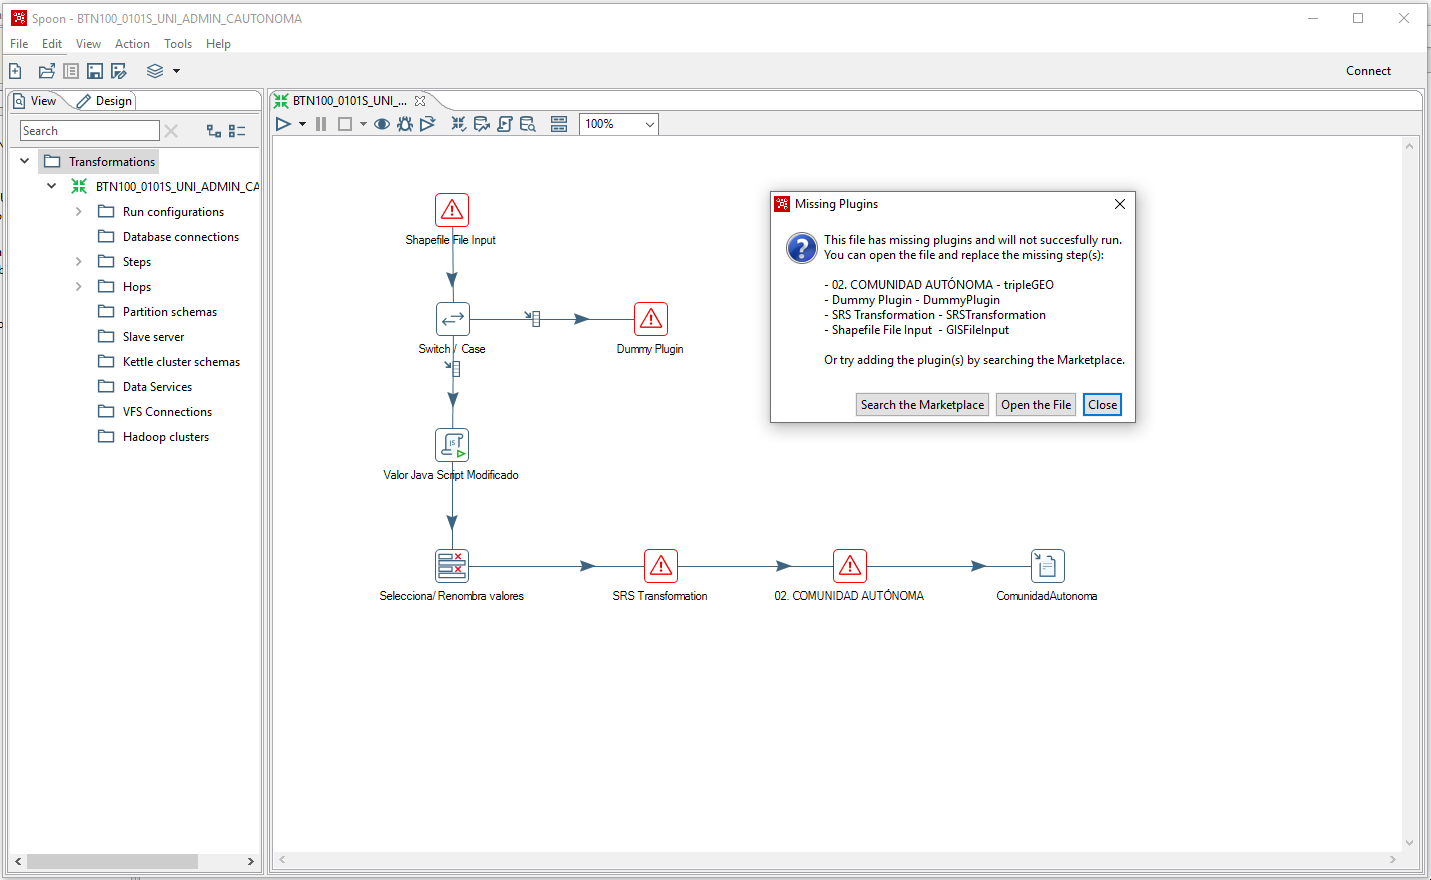
\includegraphics[width=\textwidth]{images/spoon-missing-plugins.png}
    \centering
    \caption{Transformación GEOKettle importada en la nueva suite PDI9}
    \label{fig:spoon-missing-plugins}
\end{figure}

\newpage
\subsection{Funcionamiento PDI}

Para poder realizar el ``port'' de GeoKettle a Spoon, primero es necesario entender el funcionamiento y
transformaciones actuales de GeoKettle observando la entrada y salida de cada paso. Ademas esta manera se
observara mejor el flujo de datos y sera mas fácil añadir soporte a GeoPackage en el futuro. No todas las
transformaciones tienen los mismos pasos, pero son pero todas tienen pasos en común y una estructura parecida.
Como ejemplo se utilizaran los datos de BTN100\_0101S\_UNI\_ADMIN y la transformación
BTN100\_0101S\_UNI\_ADMIN \_CAUTONOMA, ambos en la ruta /transformaciones-shape/1-UnidadesAdministrativas del
repositorio github btn100. La transformación contiene los siguientes pasos:

\begin{figure}[H]
    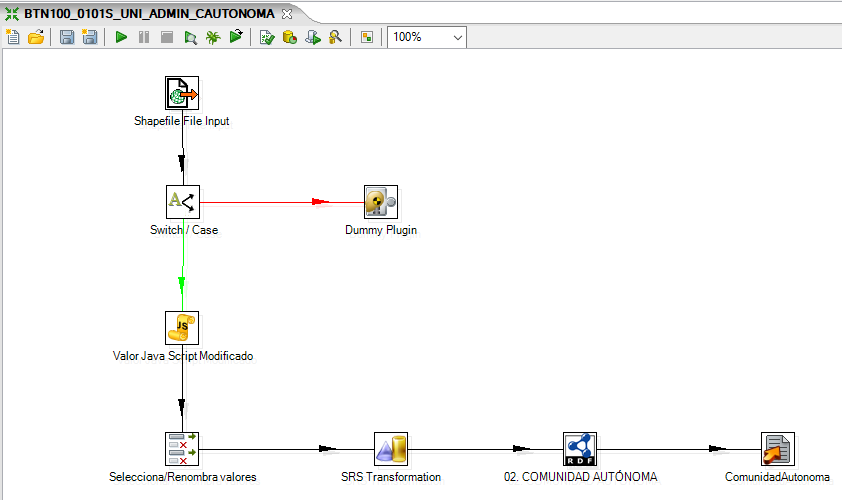
\includegraphics[width=\textwidth]{images/CCAA.png}
    \centering
    \caption{Transformación BTN100\_0101S\_UNI\_ADMIN\_CAUTONOMA}
    \label{fig:CCAA}
\end{figure}


\begin{enumerate}
    \item Shapefile File Input
    \item Switch Case
    \item Dummy Plugin
    \item Valor Java Script Modificado
    \item Selecciona/Renombra valores
    \item SRS Transformation
    \item TripleGeo
    \item Text Output
\end{enumerate}


\subsubsection{Shapefile File Input}

Lee el fichero shapefile.
\begin{enumerate}
    \item \textit{.shp}: Geometría fig.\ref{fig:shapefile}

        \begin{figure}[H]
            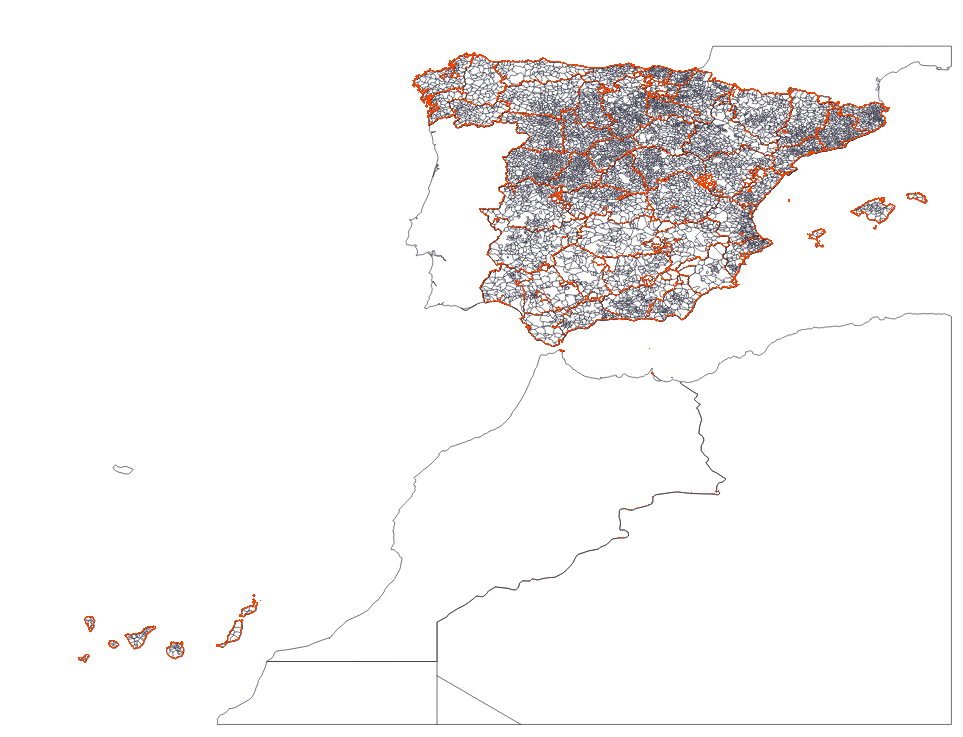
\includegraphics[width=0.7\textwidth]{images/shapefile.png}
            \centering
            \caption{Geometría contenida en el shapefile}
            \label{fig:shapefile}
        \end{figure}

    \item \textit{.dbf}: Datos asociados en columnas fig.\ref{fig:dbf}

        \begin{figure}[H]
            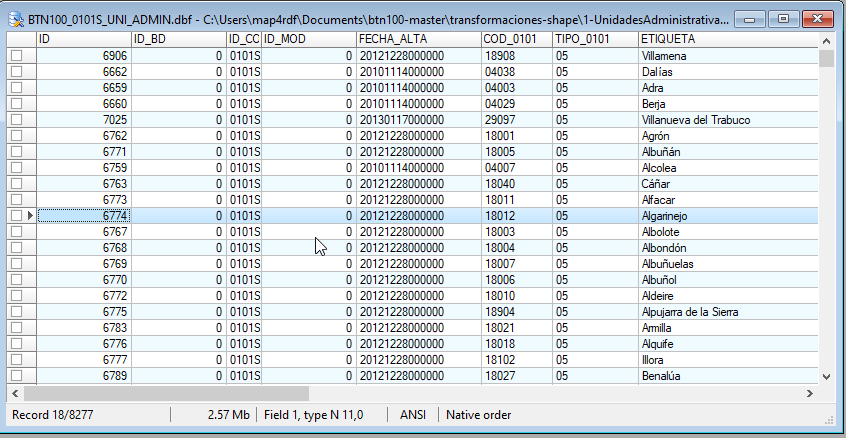
\includegraphics[width=0.7\textwidth]{images/dbf.png}
            \centering
            \caption{Datos columnares dbf asociados a la geometría}
            \label{fig:dbf}
        \end{figure}

    \item \textit{.shx}: Índice para acelerar búsquedas
    \item \textit{.prj}: Sistema de coordenadas
\end{enumerate}

\subsubsection{Switch case}
El switch case se encarga de filtrar y seleccionar las comunidades autónomas, identificadas por el valor 02 del
Campo TIPO\_0101. Si son una CCAA, se envían al paso 4, en otro caso, se envían al paso 3. fig.\ref{fig:switch} y
\ref{fig:tipo02}

\begin{figure}[H]
    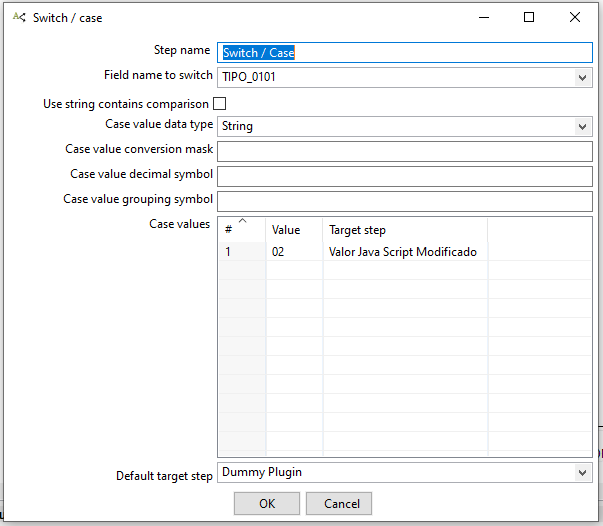
\includegraphics[width=0.7\textwidth]{images/switch.png}
    \centering
    \caption{Paso switch}
    \label{fig:switch}
\end{figure}

\begin{figure}[H]
    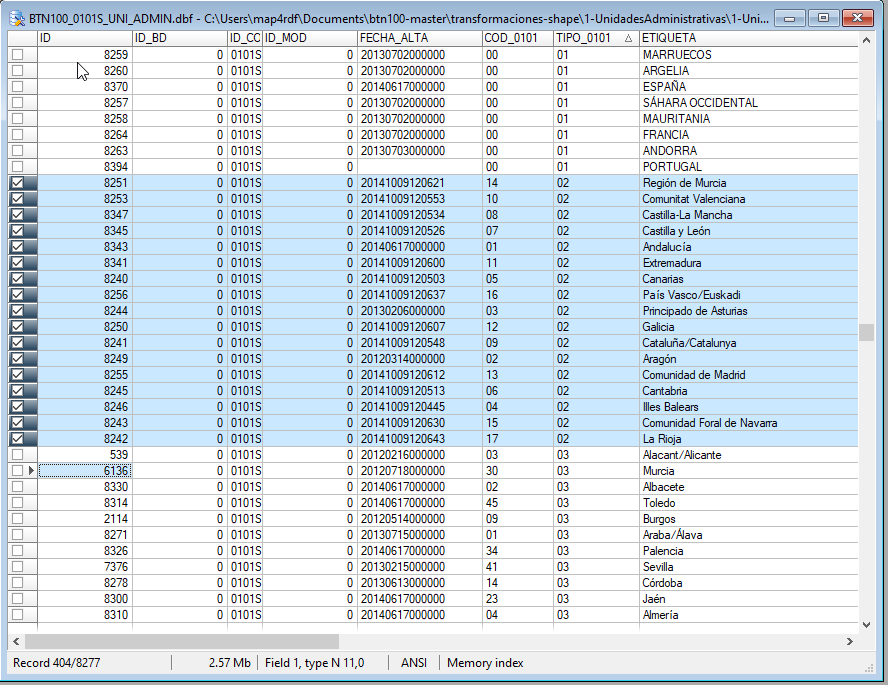
\includegraphics[width=\textwidth]{images/tipo02.png}
    \centering
    \caption{La filas correspondientes a las CCAA}
    \label{fig:tipo02}
\end{figure}

\subsubsection{Dummy Plugin}
No hace ninguna transformación, su propósito es recoger los datos innecesarios del switch.

\subsubsection{Valor JavaScript Modificado}
El script cambia el formato de la fecha para facilitar la lectura: de YYYYMMDDHHMMSS a YYYY-MM-DD. También
crea un nuevo campo llamado identificador a partir del campo etiqueta, cambiando espacios por barras bajas, mayúsculas
por minúsculas, quitando tildes y signos de puntuación. fig.\ref{fig:script} y \ref{fig:fecha}

\begin{figure}[H]
    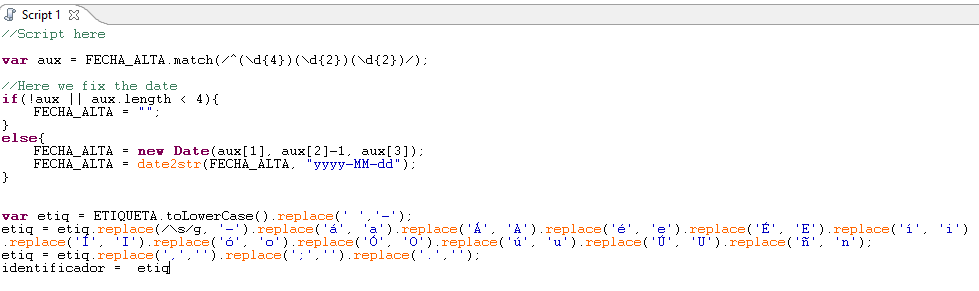
\includegraphics[width=\textwidth]{images/script.png}
    \centering
    \caption{Script Javascript}
    \label{fig:script}
\end{figure}

\begin{figure}[H]
    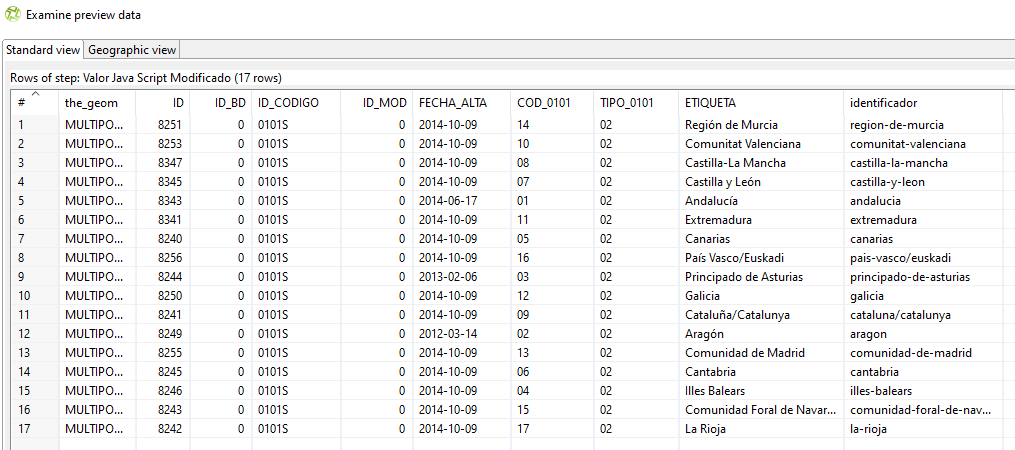
\includegraphics[width=\textwidth]{images/fecha.png}
    \centering
    \caption{Resultado del cambio de formato de fecha}
    \label{fig:fecha}
\end{figure}

\subsubsection{Selecciona/Renombra valores}
Cambia los metadatos de la columna FECHA\_ALTA para que sea reconocida como fecha. fig.\ref{fig:selecciona-renombra}

\begin{figure}[H]
    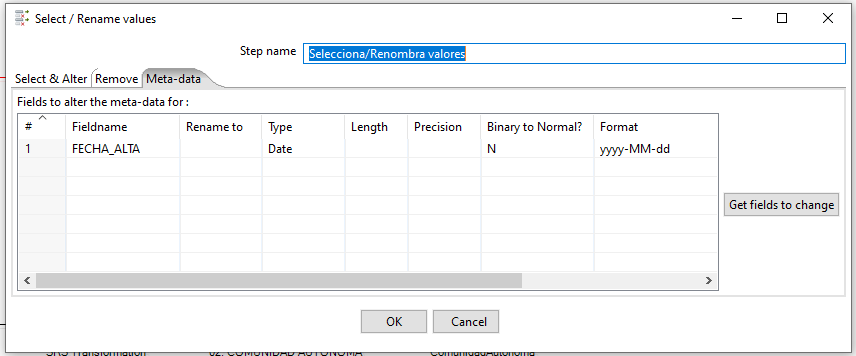
\includegraphics[width=\textwidth]{images/selecciona-renombra.png}
    \centering
    \caption{Selecciona/renombra valores}
    \label{fig:selecciona-renombra}
\end{figure}

\subsubsection{SRS Transformation}
Realiza la reproyección del sistema de coordenadas de ETRS89 a WGS84. fig.\ref{fig:SRS}

\begin{figure}[H]
    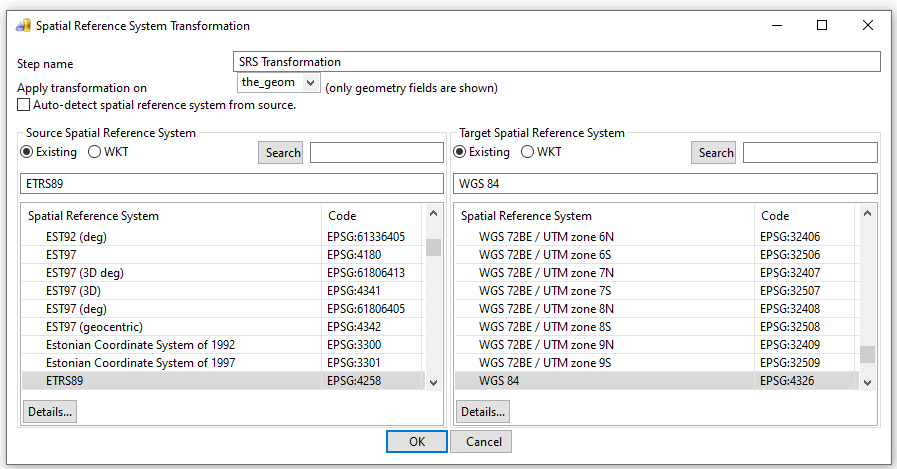
\includegraphics[width=\textwidth]{images/SRS.png}
    \centering
    \caption{Transformación SRS}
    \label{fig:SRS}
\end{figure}

\subsubsection{TripleGeoKettle}
Transforma el shapefile del paso anterior en RDF en formato .ttl (Turtle). Se pueden configurar los parámetros asociados a la
ontología y decidir si se muestran ciertas columnas o no. fig.\ref{fig:tripleGeoKettle}


\begin{figure}[H]
    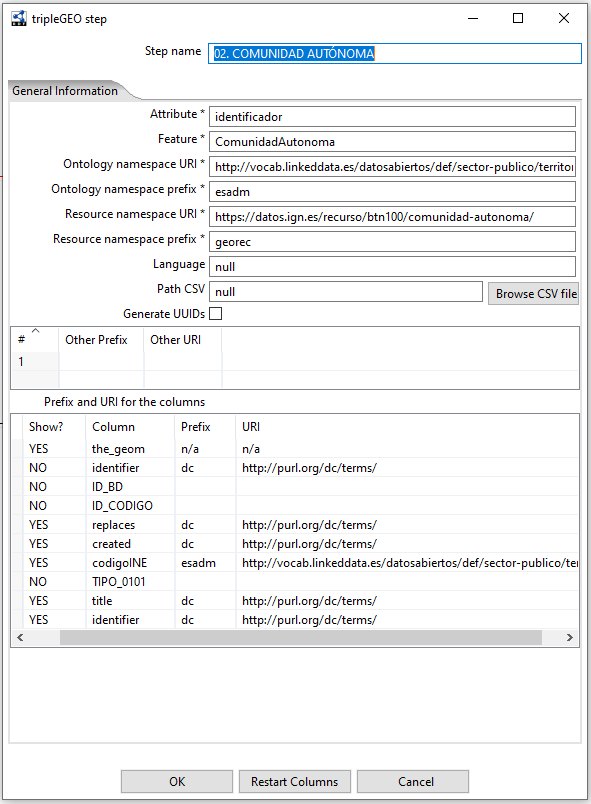
\includegraphics[width=0.9\textwidth]{images/tripleGeoKettle.png}
    \centering
    \caption{tripleGeoKettle}
    \label{fig:tripleGeoKettle}
\end{figure}

\subsubsection{Text file output}
Escribe los datos RDF en un fichero de texto con formato .ttl. fig.\ref{fig:text-file-output}
\begin{figure}[H]
    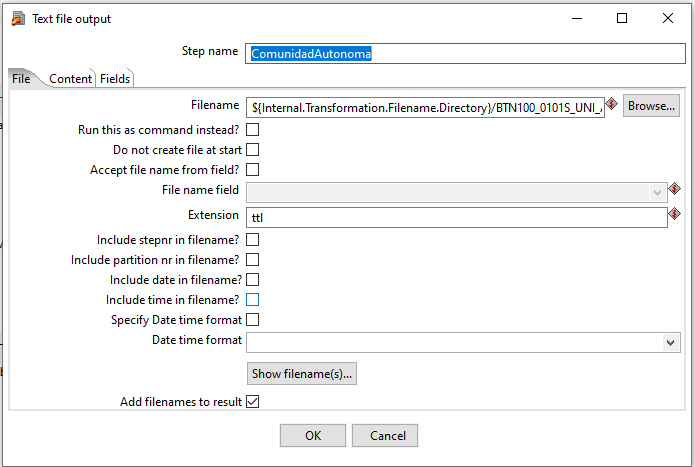
\includegraphics[width=\textwidth]{images/text-file-output.png}
    \centering
    \caption{text-file-output}
    \label{fig:text-file-output}
\end{figure}

\subsubsection{Resultado de la transformación}
\footnotesize
\begin{verbatim}
@prefix geo:   <http://www.w3.org/2003/01/geo/wgs84_pos#> .
@prefix geosparql: <http://www.opengis.net/ont/geosparql#> .
@prefix sf:    <http://www.opengis.net/ont/sf#> .
@prefix rdf:   <http://www.w3.org/1999/02/22-rdf-syntax-ns#> .
@prefix owl:   <http://www.w3.org/2002/07/owl#> .
@prefix xsd:   <http://www.w3.org/2001/XMLSchema#> .
@prefix georec: <https://datos.ign.es/recurso/btn100/comunidad-autonoma/> .
@prefix esadm: <http://vocab.linkeddata.es/datosabiertos/def/sector-publico/territorio#> .
@prefix rdfs:  <http://www.w3.org/2000/01/rdf-schema#> .
@prefix foaf:  <http://xmlns.com/foaf/0.1/> .
@prefix dc:    <http://purl.org/dc/terms/> .

georec:comunidad-de-madrid
        a                      esadm:ComunidadAutonoma ;
        rdfs:label             "comunidad-de-madrid" ;
        dc:created             "2014-10-09"^^xsd:date ;
        dc:identifier          "comunidad-de-madrid" ;
        dc:title               "Comunidad de Madrid" ;
        esadm:codigoINE        "13"^^xsd:int ;
        geosparql:hasGeometry  <https://datos.ign.es/recurso/btn100/comunidad-autonoma/...

georec:region-de-murcia
        a                      esadm:ComunidadAutonoma ;
        rdfs:label             "region-de-murcia" ;
        dc:created             "2014-10-09"^^xsd:date ;
        dc:identifier          "region-de-murcia" ;
        dc:title               "Region de Murcia" ;
        esadm:codigoINE        "14"^^xsd:int ;
        geosparql:hasGeometry  <https://datos.ign.es/recurso/btn100/comunidad-autonoma/...

<https://datos.ign.es/recurso/btn100/comunidad-autonoma/aragon/geometry>
        a                sf:Polygon ;
        geosparql:asWKT  "POLYGON ((-1.6174492000010632 40.94373283914169, -1.62366030000...
        ...
\end{verbatim}
\normalsize


\section{Port a PDI9}

\subsection{Tests con pentaho-gis-plugins}

El 3 de Marzo de 2021 el plugin añadió soporte para el formato GeoPackage. Con el siguiente test se comprueba que los
pasos o steps que se utilizaran para reemplazar las transformaciones antiguas funcionan correctamente.

\begin{figure}[H]
    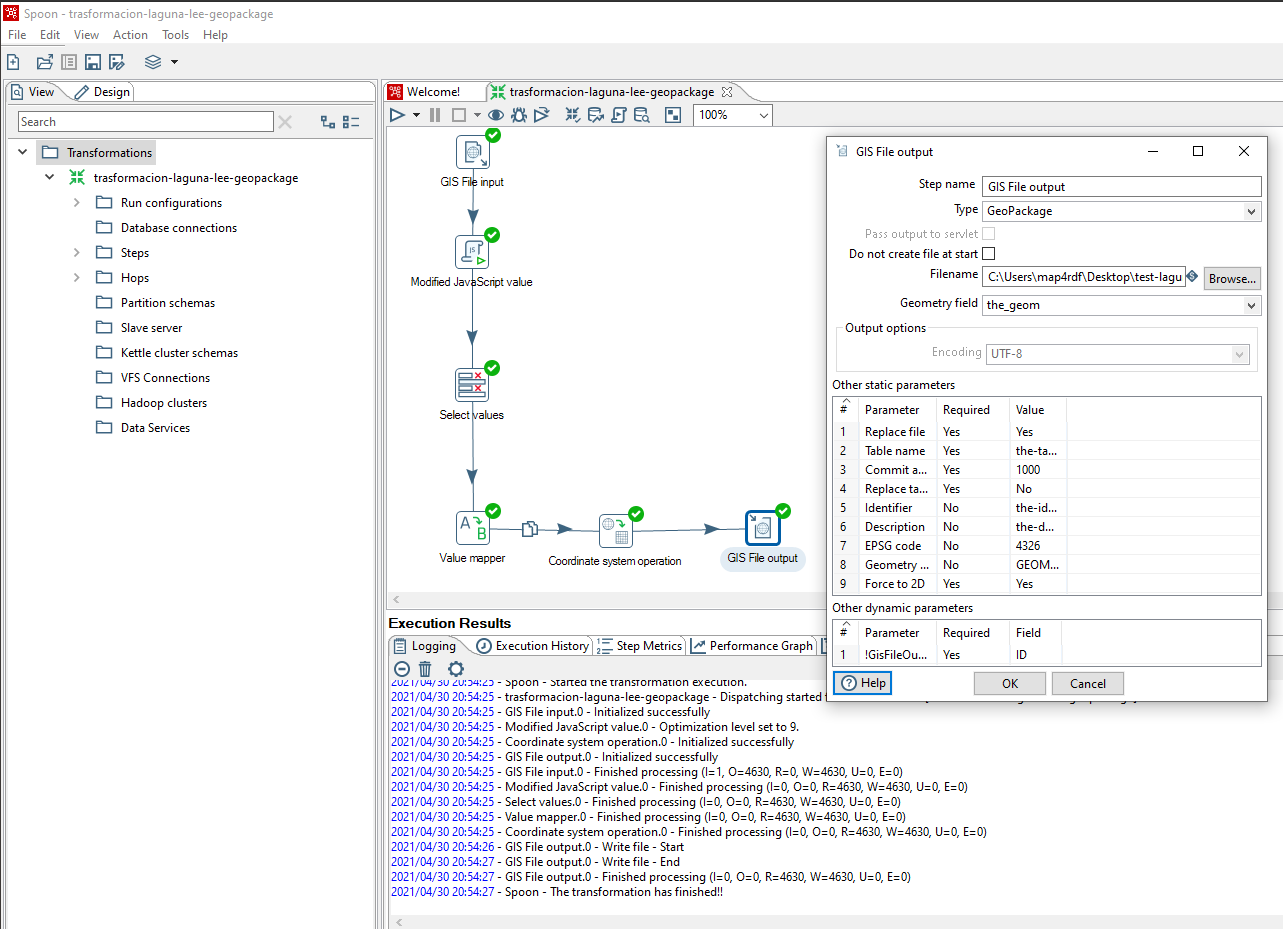
\includegraphics[width=\textwidth]{images/test-laguna-geopackage.png}
    \centering
    \caption{test-laguna-geopackage}
    \label{fig:test-laguna-geopackage}
\end{figure}

\subsection{Entorno de desarrollo}

\subsubsection{Dependencias e instalación}

En los últimos años Pentaho ha pasado de utilizar Apache Ant a utilizar Apache Maven. TripleGeoKettle también
utilizaba Ant, y se ha decidido utilizar Maven por las ventajas que ofrece. El proyecto TripleGeoKettle contenía
una carpeta lib en la que se encontraban los .jar con las dependencias necesarias. Ahora, las dependencias se
administran con Maven y el pom.xml. Para ello se incluyen los repositorios de Pentaho y OSGeo y las dependencias
que se quieren incluir. Las properties funcionan a modo de ``variable'' para poder cambiar la versión de pdi
fácilmente en un solo lugar. maven-assembly-plugin compila el plugin y genera el .jar.


\lstinputlisting[language=XML]{code/pom-old.xml}

A continuación se muestran los pasos para configurar el entorno de desarrollo en Arch Linux:

\begin{lstlisting}
# Instalar PDI desde AUR (los mirrors son mucho mas rapidos que los de SourceForge)
yay -S pdi-ce
# Instalar Java 8
sudo pacman -S jdk8-openjdk
# Cambiar la version de java con
sudo archlinux-java set java-8-openjdk
# Instalar el Plugin de desarrollo
https://sourceforge.net/projects/pentaho/files/Pentaho%209.1/plugins/kettle-sdk-plugin-assembly-9.1.0.0-324.zip/download
# Instalar Maven
sudo pacman -S maven
# Descargar el settings.xml del repositorio de github en ~/.m2
https://raw.githubusercontent.com/pentaho/maven-parent-poms/master/maven-support-files/settings.xml
# Desde el directorio del plugin compilar y empaquetar el plugin
mvn clean package
# Instalarlo en PDI9 copiando el contenido del .zip generado en el directorio target
sudo cp target/tripleGeoKettle-oeg-1.jar /opt/pdi/plugins/steps/tripleGeoKettle-oeg-1/
\end{lstlisting}

\subsubsection{Pentaho sdk plugins}

Pentaho ofrece plugins\cite{pdi-sdk} muy sencillos de ejemplo que muestran como implementar un plugin. Para el
port de TripleGeoKettle se ha utilizado como referencia kettle-sdk-step-plugin, que simplemente escribe Hello
World. Con él se ha probado la compilación, el pom.xml customizado, y se han realizado pruebas varias como
cambiar el icono o el nombre del plugin.


\section{Proceso de porteo}

\subsection{Diseño del plugin}



Se comienza con el sdk de Pentaho y se realizan los cambios necesarios para integrar TripleGeoKettle en el nuevo
entorno. Se muestran las imágenes del antes y después de la estructura de carpetas. fig.\ref{fig:directorios-sdk}
y \ref{fig:directorios-TGK}

\begin{figure}[H]
    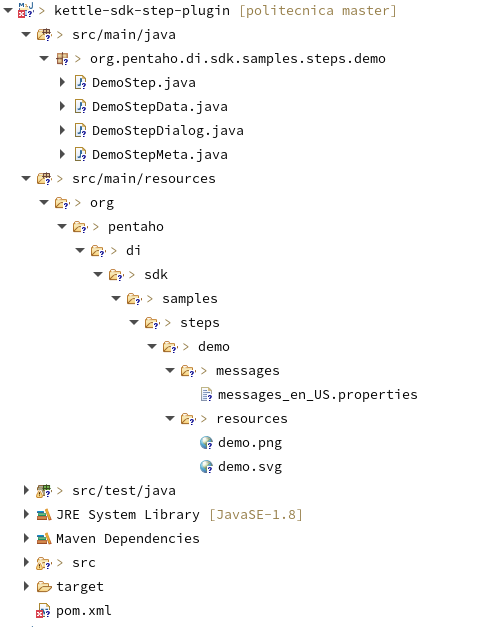
\includegraphics[width=0.7\textwidth]{images/directorios-sdk.png}
    \centering
    \caption{Estructura de carpetas del sdk}
    \label{fig:directorios-sdk}
\end{figure}

\begin{figure}[H]
    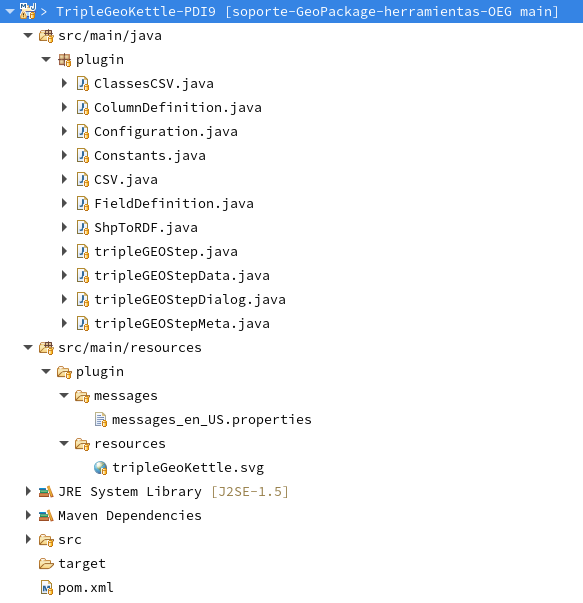
\includegraphics[width=0.7\textwidth]{images/directorios-TGK.png}
    \centering
    \caption{Estructura de carpetas de TripleGeoKettle portado}
    \label{fig:directorios-TGK}
\end{figure}

\textbf{Pasos seguidos:}

\begin{enumerate}
    \item Cambiar el nombre del paquete a ``plugin''. Es importante que el de java y el de resources tengan el
        mismo nombre para que los diálogos lean el fichero properties correctamente.

    \item Actualizar el fichero messages.properties, que contiene el texto de la GUI del plugin y varios enlaces.
\begin{lstlisting}
#sdk properties
tripleGEO.FieldName.Label=Output field name
tripleGEO.CheckResult.ReceivingRows.OK=Step is receiving input from other steps.
tripleGEO.CheckResult.ReceivingRows.ERROR=No input received from other steps!

tripleGEOStep.Name=TripleGeoKettle
tripleGEOStep.TooltipDesc=An ETL Tool for Transforming Geospatial Data into RDF under the GeoSPARQL standard.
tripleGEOStep.DocumentationURL=https://github.com/oeg-upm/geo.linkeddata.es-TripleGeoKettle/wiki
tripleGEOStep.CasesURL=https://github.com/oeg-upm/geo.linkeddata.es-TripleGeoKettle/issues
tripleGEOStep.ForumURL=https://github.com/oeg-upm/geo.linkeddata.es-TripleGeoKettle/issues
tripleGEOStep.Linenr=Linenr {0}
tripleGEOStep.Error.NoOutputField=Could not find Output Field in row

# tripleGeoKettle custom properties
tripleGEOStepDialog.Shell.Title=tripleGEO step
tripleGEOStepDialog.Tab.MainTab=General Information
tripleGEOStepDialog.AttributeName.Label=Attribute *
tripleGEOStepDialog.Feature.Label=Feature *
tripleGEOStepDialog.OntologyNS.Label=Ontology namespace URI *
tripleGEOStepDialog.OntologyNSPrefix.Label=Ontology namespace prefix *
tripleGEOStepDialog.ResourceNS.Label=Resource namespace URI *
tripleGEOStepDialog.ResourceNSPrefix.Label=Resource namespace prefix *
tripleGEOStepDialog.Language.Label=Language
tripleGEOStepDialog.PathCSV.Label=Path CSV
tripleGEOStepDialog.PathCSVButton.Label=Browse CSV file
tripleGEOStepDialog.PathCSVButtonTooltip.Label=Browse for CVS file
tripleGEOStepDialog.uuids.Label=Generate UUIDs
tripleGEOStepDialog.Fields.Label=Other prefix and URI
tripleGEOStepDialog.other.Label=Other URI
tripleGEOStepDialog.otherPrefix.Label=Other Prefix
tripleGEOStepDialog.Column.Label=Column
tripleGEOStepDialog.Columns.Label=Prefix and URI for the columns
tripleGEOStepDialog.otherColumns.Label=URI
tripleGEOStepDialog.otherPrefixColumns.Label=Prefix
tripleGEOStepDialog.ShowColumns.Label=Show?
tripleGEOStepDialog.RestartFields.Button=Restart Columns
\end{lstlisting}

    \item Modificar la annotation @Step de DemoStepMeta.java. Se utiliza para que el programa reconozca y
        categorice el plugin correctamente.
\begin{lstlisting}
@Step(
   id = "TripleGeoKettle",
   name = "tripleGEOStep.Name",
   description = "tripleGEOStep.TooltipDesc",
   image = "plugin/resources/tripleGeoKettle.svg",
   categoryDescription = "i18n:org.pentaho.di.trans.step:BaseStep.Category.Transform",
   i18nPackageName = "tripleGeoKettle",
   documentationUrl = "tripleGEOStep.DocumentationURL",
   casesUrl = "tripleGEOStep.CasesURL",
   forumUrl = "tripleGEOStep.ForumURL"
   )
\end{lstlisting}

    \item Cambiar los nombres de las clases de Demo a TripleGeoKettle.
    \item Importar las clases java auxiliares de tripleGeoKettle.
    \item Existe un método deprecado en tripleGeoStepMeta.java: Valuemeta(). Se utiliza el constructor sin
        parámetros y luego se le asigna el tipo 2. Para sustituirlo, como el tipo es 2, que según la siguiente
        tabla\cite{tabla-string} significa string, es necesario cambiarlo a ValueMetaString().

    \item Error en los métodos readRep y saveRep. Es necesario importar ObjectId
         y sustituir el tipo long por ObjectId en la cabecera de la función.

    \item Cambiar la siguiente línea para que la clase Dialog lea correctamente los contenidos del fichero
        properties.

    \begin{lstlisting}
    main/java/plugin/tripleGEOStepDialog.java:69
    private static String PKG = tripleGEOStepDialog.class.getPackage().getName();
    \end{lstlisting}

\item PDI9 utiliza iconos .svg y proporciona una guia de diseño\cite{guia-diseno}. Por tanto se ha actualizado el
    icono antiguo de .png a .svg con los nuevos colores fig.\ref{fig:icono-TGK}
\end{enumerate}

\begin{figure}[H]
  \centering
    \includesvg{../TripleGeoKettle-PDI9/src/main/resources/plugin/resources/tripleGeoKettle.svg}
    \caption{Nuevo icono svg}
    \label{fig:icono-TGK}
    \centering
\end{figure}

\subsection{Resultado parcial}

La base del porteo se ha realizado correctamente como se puede ver en la figura \ref{fig:TGK-portado}. El dialogo
se abre y se pueden cambiar los parámetros de configuración. También es capaz de leer la salida del paso anterior
de SRS. Sin embargo, todavía no funciona correctamente. Probablemente se debe a que el paso
anterior (transformación de coordenadas) pasa su información de manera distinta al de GeoKettle (en PDI le llegan
9 campos y en GeoKettle 8). Sera necesario seguir los pasos de la documentación para conectar el debugger y solucionar el
problema de NullPointerException.

\begin{figure}[H]
    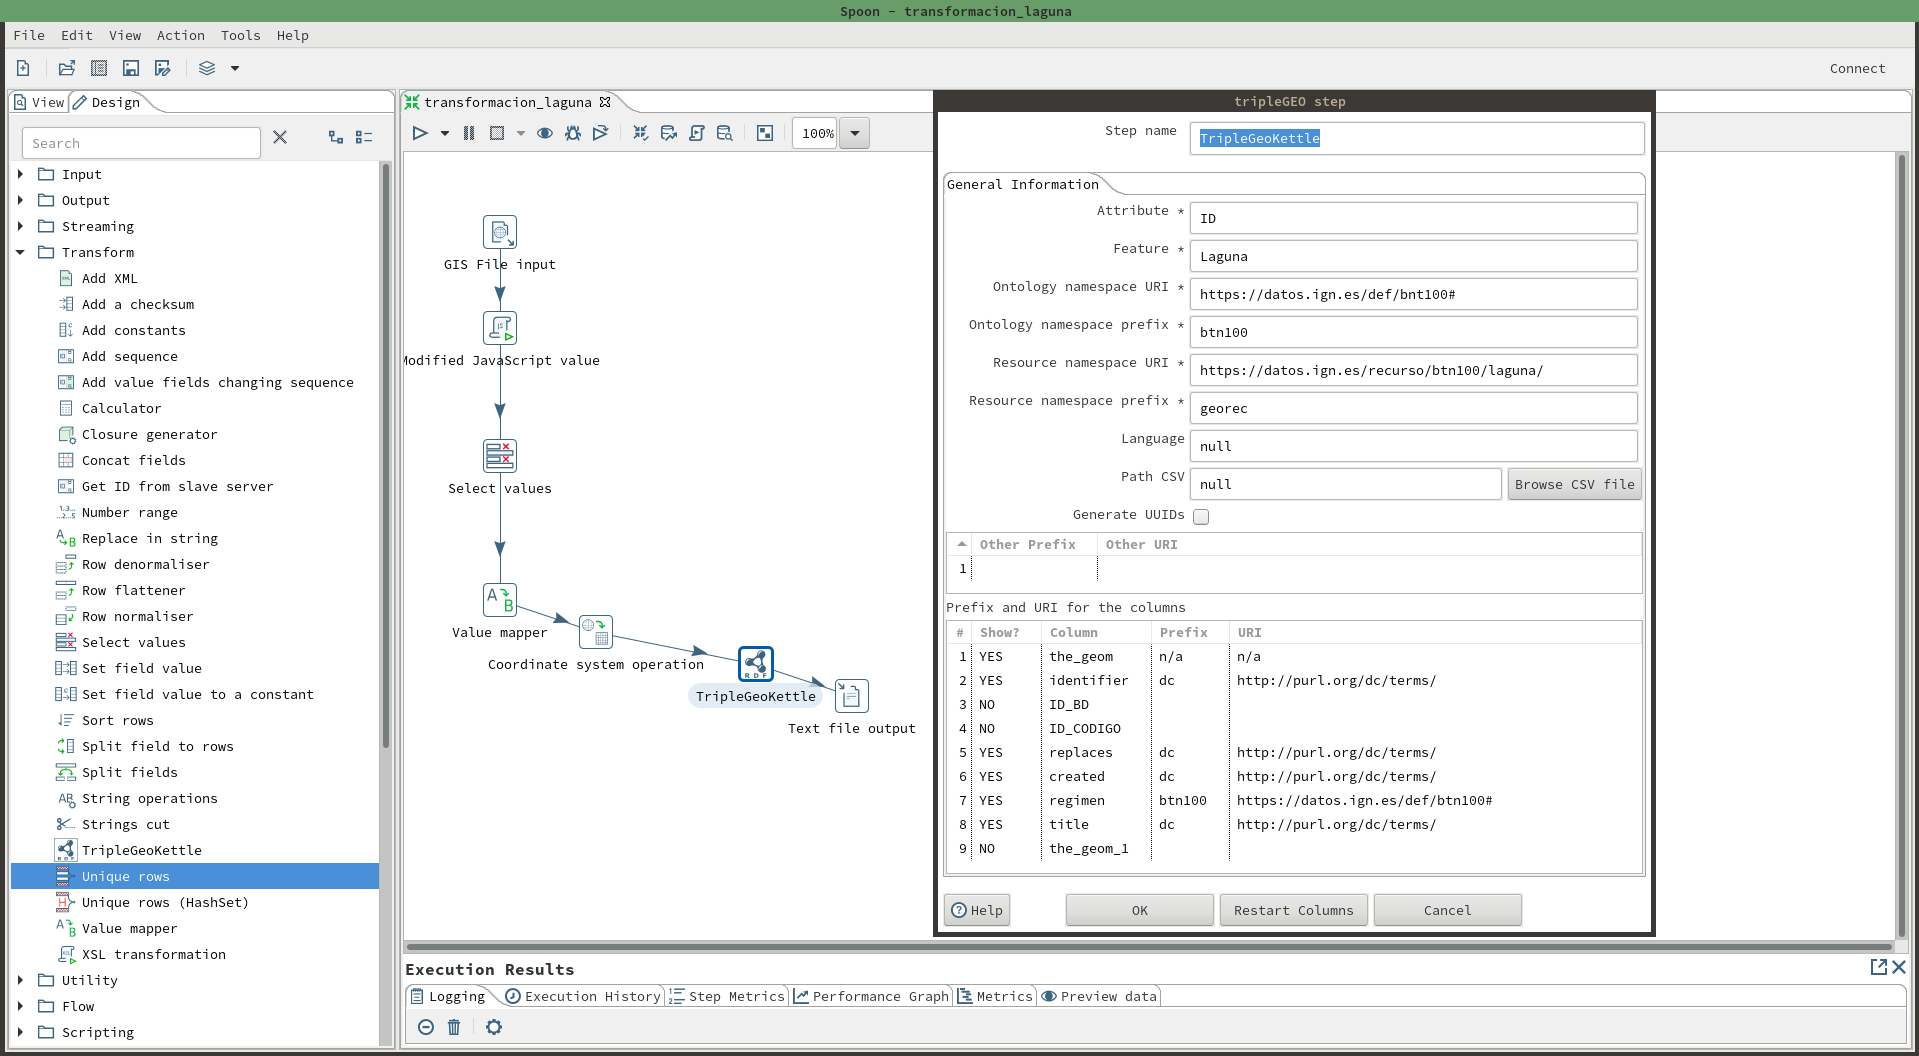
\includegraphics[width=\textwidth]{images/TGK-portado.png}
    \centering
    \caption{TripleGeoKettle corriendo en PDI9}
    \label{fig:TGK-portado}
\end{figure}


\subsection{Debugging}

Para depurar el plugin se ha creado una nueva configuración de depuración eclipse en localhost y el puerto 1044
(fig.\ref{fig:debug-configurations}). Por otro lado se ha creado una copia del script de inicio de PDI9 spoon.sh,
llamada debug-spoon.sh, y se le han añadido los siguientes parámetros de ejecución.

\newpage
\begin{lstlisting}
if [ -z "\$PENTAHO_DI_JAVA_OPTIONS" ]; then
    PENTAHO_DI_JAVA_OPTIONS="-Xms1024m -Xmx2048m -Xdebug -Xnoagent -Djava.compiler=NONE -Xrunjdwp:transport=dt_socket,server=y,suspend=y,address=1044"
fi
\end{lstlisting}

\begin{figure}[H]
    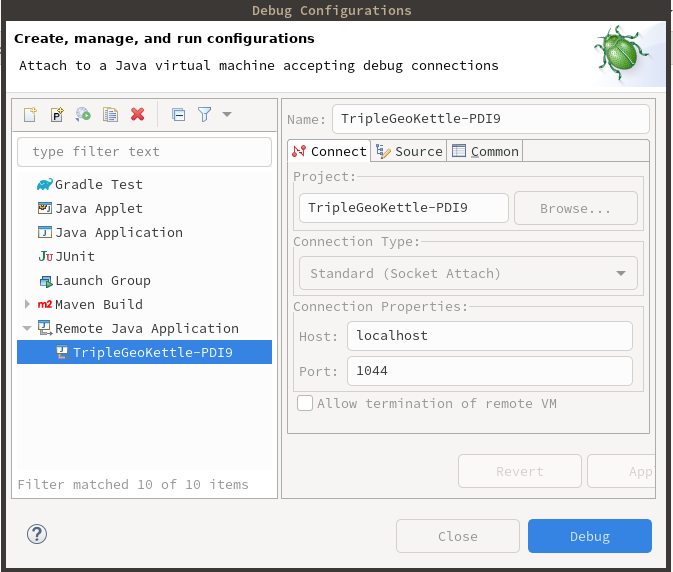
\includegraphics[width=\textwidth]{images/debug-configurations.png}
    \centering
    \caption{Configuración de depuración en Eclipse}
    \label{fig:debug-configurations}
\end{figure}

El trazado del error NullPointerException obtenido tras ejecutar la transformación es el siguiente:

\begin{lstlisting}
1. Con la siguiente llamada se inicia el modelo RDF:
    tripleGEOStep.java 160: this.shpToRDF.getModelFromConfiguration();

2. Desde la funcion se crea el modelo con:
    Model modelAux = ModelFactory.createOntologyModel(OntModelSpec.RDFS_MEM);

3. En ese momento salta una exception que no detiene el programa y la variable modelAux se mantiene en null.
    Schema factory class org.apache.xerces.impl.dv.xs.SchemaDVFactoryImpl does not extend from SchemaDVFactory.

4. Despues se utiliza en la funcion
    ShpToRDF.java 176: setModel_rdf(modelAux);

5. Y como modelAux se ha inicializado a null, model_rdf tambien lo es.
    ShpToRDF.java 712: public void setModel_rdf(Model model_rdf) { this.model_rdf = model_rdf; }

6. Finalmente, al llamar a la siguiente funcion salta NullPointerException ya que model_rdf es null:
ShpToRDF.java 550:
	private void insertResourceTypeResource(String r1, String r2) {
		this.model_rdf.add(this.model_rdf.createResource(r1), RDF.type, this.model_rdf.createResource(r2));
	}


\end{lstlisting}
La causa es una incompatibilidad de dependencias.
Apache Jena y vividsolutions.jts utilizan Xerces, pero versiones distintas.



\subsection{Problemas de dependencias}

Para el pom.xml de Maven se ha decidido dejar de utilizar maven-assembly-plugin ya que en algunos casos no
incluía los jars necesarios y saltaban errores en tiempo de ejecución. En su lugar se utilizará
maven-shade-plugin que es más apropiado para proyectos grandes con muchas dependencias que pueden tener
conflictos entre sí. Además crea un ``super jar'' que incluye todas las dependencias, tal y como se hacía antiguamente
con el build.xml de Ant.

Las versiones detalladas en el pom.xml son necesarias por compatibilidad. Por ejemplo, no es posible utilizar la
versión de jts que se utilizaba anteriormente (1.11), ni la de gt-geometry, ya que hay muchos problemas de compatibilidad debido a
Xerces. Xerces también se utiliza en Jena, y debido a que todas las dependencias (incluso las de pentaho) utilizan
Xerces, ha sido un verdadero rompecabezas solucionar las incompatibilidades. Es más, fue tan complicado, que
durante unos días se pasó todo el código de Jena del fichero ShpToRDF.java a otra librería (RDF4J) para evitar
las incompatibilidades. Pero como llevó al detenido estudio del código fuente, ayudó a encontrar las
incompatibilidades que tenía Jena con Xerces y los métodos deprecados.

Fue necesario realizar dos cambios: 

\begin{lstlisting}
ShpToRDF:347, debido al error de cast, cambiar
    geometry = reader.read((String)row[this.posGeometry]);
por 
    geometry = reader.read(row[this.posGeometry].toString());

tripleGEOStep:73, debido a error unsupported operationexception, cambiar
    rm.remove(0)
por
    rm.removeValueMeta(0);
\end{lstlisting}

Finalmente el contenido del pom.xml es el siguiente:

\lstinputlisting[language=XML]{../TripleGeoKettle-PDI9/pom.xml}


\section{Adaptación de las transformaciones}

Una vez el plugin ha sido porteado, el siguiente paso es adaptar todas las transformaciones .ktr para que puedan
ejecutarse en PDI9. La mayoría de los pasos existentes se pueden copiar y pegar directamente desde
GeoKettle a PDI9 (switch/case, valor javascript modificado, salida de fichero de texto, selecciona/renombra
valores, filtrar...). Es necesario sustituir el paso que lee el fichero shp y el de transformación de coordenadas
por los respectivos de pentaho-gis-plugins. El paso de GeoKettle no hace falta modificarlo, pero hace falta
precederlo por un paso de seleccionar/renombrar valores, ya que además de la geometría transformada, el paso de
SRS nuevo también pasa la geometría original. Es necesario quitar la original del pipeline y sustituirla por la
original en el mismo orden para que GeoKettle la lea sin problemas. El modo de trabajo ha sido el siguiente para
los 104 ficheros .ktr:

\begin{enumerate}
    \item Crear la nueva transformación
    \item Copiar los pasos compatibles de GeoKettle a PDI9 (Ctrl+C,V)
    \item Añadir los 3 pasos nuevos (input, transformación, renombrado)
    \item Ejecutar la transformación y comprobar que los ficheros output coinciden con los originales.
\end{enumerate}

Fue considerado realizar estos cambios mediante un script, pero las transformaciones no son homogéneas, algunas
tienen unos pasos y otras no, y por tanto habría sido necesario revisarlas todas manualmente. Por tanto, hacer
las transformaciones se ha considerado más rápido y seguro.

\begin{figure}[H]
    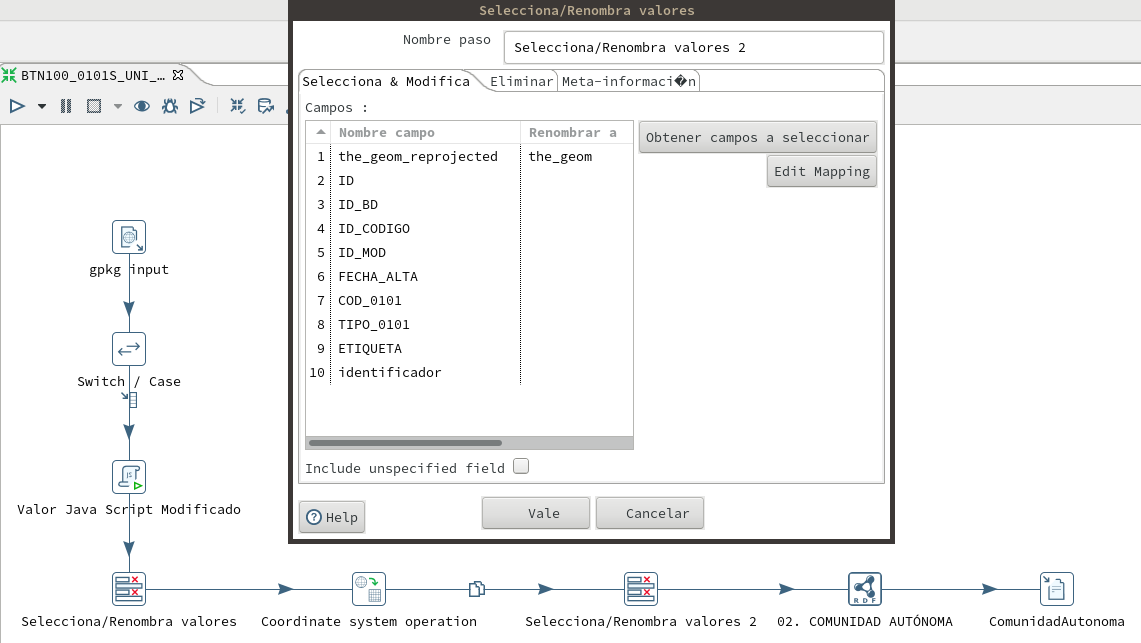
\includegraphics[width=\textwidth]{images/renombra-geom.png}
    \centering
    \caption{Nuevos pasos y renombrado/reordenado de los valores}
    \label{fig:renombra-geom}
\end{figure}

\section{Soporte GeoPackage}

El primer paso para añadir soporte a GeoPackage es convertir todos los .shp y ficheros relacionados a .gpkg. Para
ello se hace uso del comando ogr2ogr de GDAL\cite{ogr2ogr}. El parámetro -nln Table es el nombre de la capa de
geometría, que debe coincidir con el del step gpkg input.

A continuación se modifica el primer step de la transformación, el de lectura de .shp a .gpkg, utilizando
sustituciones sed en el en el .ktr, ya que en el fondo es un fichero .xml.

Todo esto lo realiza el script shpTogpkg.sh:

\lstinputlisting[language=BASH]{../scripts/shpTogpkg.sh}



A continuación, es necesario volver a ejecutar todas las transformaciones y comprobar que los resultados son los
mismos que con los .shp. Mediante el script gpkg-tests.sh es ejecutan las transformaciones con la herramienta
pan de pentaho y se comparan los ficheros .ttl originales con los recién generados.

\lstinputlisting[language=BASH]{../scripts/gpkg-tests.sh}

\section{Problemas encontrados}

\subsection{Out of memory}
Al ejecutar varias transformaciones se genera el error outofmemoryerror. Para solucionarlo, es necesario añadir
el parámetro -Xmx6g a la línea 250 de spoon.sh, como indica la gúia de pentaho \cite{outofmemory}. Simplemente
aumenta el límite de memoria que puede utilizar el programa.

\subsection{Línea eléctrica}
El archivo de transformación original BTN100\_0702L\_LIN\_ELEC.ktr era incorrecto. En el paso switch/case no se hacía
correctamente la división entre líneas de alta y baja tensión; en los dos case dejaba pasar el los mismos valores
(01) que corresponden a líneas de baja tensión. Deben dividirse entre 01 y 02.

\begin{figure}[H]
    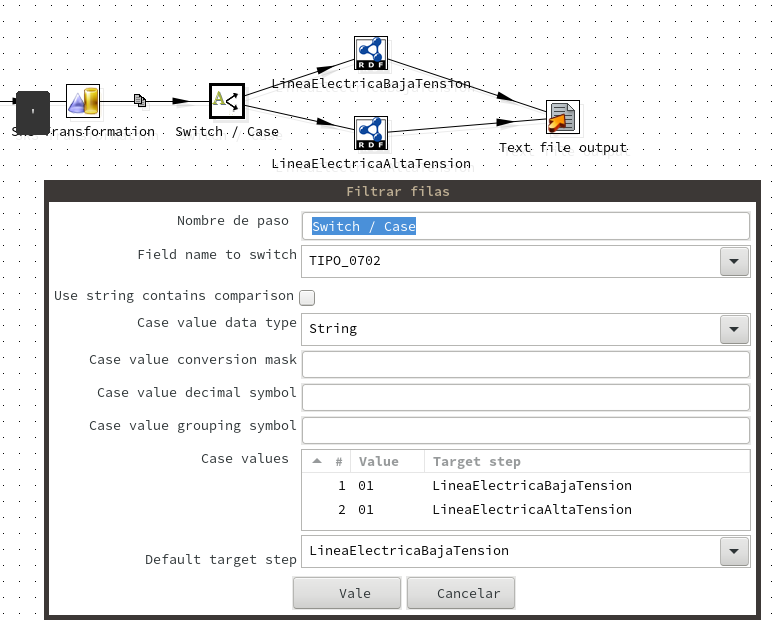
\includegraphics[width=\textwidth]{images/linea-electrica-orig.png}
    \centering
    \caption{Transformación original incorrecta}
    \label{fig:linea-electrica-orig}
\end{figure}

\begin{figure}[H]
    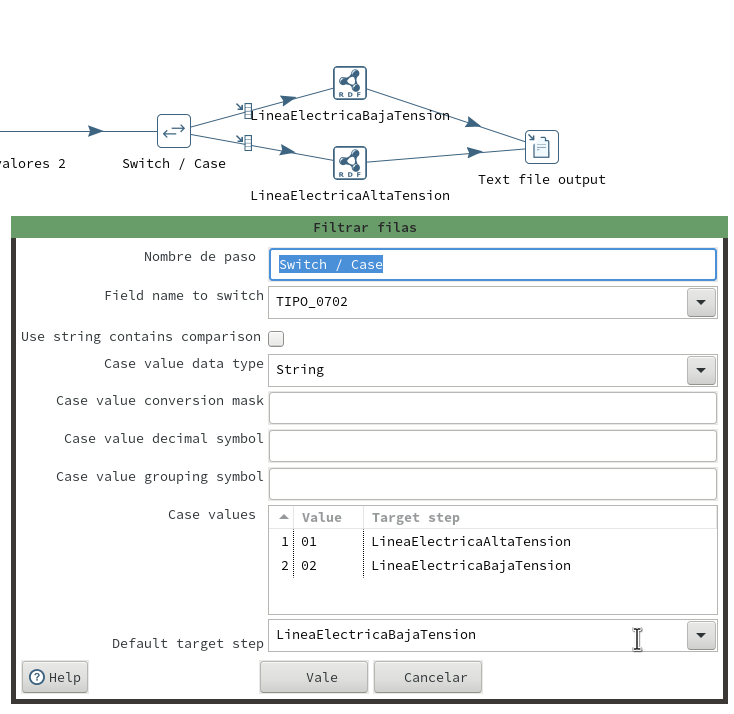
\includegraphics[width=\textwidth]{images/linea-electrica-new.png}
    \centering
    \caption{Transformación corregida}
    \label{fig:linea-electrica-new}
\end{figure}

